\documentclass[a4paper,11pt]{article}
\usepackage{sbpo-template}
%\usepackage[latin1]{inputenc}
\usepackage[brazil]{babel}    % português do Brasil
\usepackage[utf8]{inputenc}   % acentos no UTF-8
\usepackage[T1]{fontenc}      % para hifenização correta
\usepackage{amsmath,amssymb}
\usepackage{url}
\usepackage[square]{natbib}
\usepackage{indentfirst}
\usepackage{fancyhdr}
\usepackage{graphicx}
\graphicspath{{./}{../img/}}
\usepackage{xcolor}
\usepackage{booktabs}
\pagestyle{fancy}
\fancyhf{}
\fancyhead[C]{
\includegraphics[scale=0.5]{sbpo2026-header-logo.png}}
%\renewcommand{\headrulewidth}{0pt}
\providecommand{\headruleskip}{0pt}
\renewcommand{\headruleskip}{-1mm}
%\setlength\headheight{101.0pt}
%\addtolength{\textheight}{-101.0pt}
\setlength\headheight{86pt}
\addtolength{\textheight}{-86pt}
\setlength{\headsep}{5mm}
\setlength{\footskip}{4.08003pt}

\begin{document}

\title{APLICAÇÃO DO NSGA-III NA OTIMIZAÇÃO MULTIOBJETIVO DE UM MODELO OTTO COM ADIÇÃO FINITA DE CALOR}

\maketitle
\thispagestyle{fancy}

\author{
\name{Felipe Gubaua Portes}
\institute{Universidade Tecnológica Federal do Paraná - UTFPR}
\iaddress{Av. Sete de Setembro, 3165 - Rebouças, Curitiba - PR, 80230-901}
\email{felipegubaua@alunos.utfpr.edu.br}
}

\author{
\name{Guilherme de Paula Prado}
\institute{Universidade Tecnológica Federal do Paraná - UTFPR}
\iaddress{Av. Sete de Setembro, 3165 - Rebouças, Curitiba - PR, 80230-901}
\email {guilhermeprado@alunos.utfpr.edu.br}
}

\vspace{8mm}
\begin{resumo}
Este trabalho aplica o NSGA-III à otimização simultânea da eficiência térmica e
da potência líquida específica de um modelo Otto com adição finita de calor,
empregando NSGA-II, MOPSO e MOEA/D como referências. Quatro decisões contínuas
são consideradas: rotação, instante de ignição, taxa de compressão e razão
biela--manivela. A implementação reproduziu, na precisão publicada, as
eficiências dos seis casos do artigo-base. Em 21 execuções por método, cada uma
com 4\,848 avaliações, o NSGA-III obteve hipervolume médio de 0,844977, 0,116\% abaixo do
NSGA-II; o MOPSO produziu a melhor execução isolada. Os quatro métodos
localizaram a mesma região de compromisso, com taxa de compressão próxima de 12
e razão biela--manivela elevada. Para refinar o NSGA-III no espaço ampliado,
definiu-se um protocolo de orçamento fixo com 36 configurações e confirmação
em sementes reservadas. A nova bateria ainda não foi executada; portanto,
nenhuma configuração refinada é recomendada. Os resultados confirmam o
conflito entre eficiência e potência, sem estabelecer superioridade estatística.
\end{resumo}

\bigskip
\begin{palchaves}
NSGA-III, Otimização Multiobjetivo, Motor Otto.

\bigskip
\noindent{Tópicos (MH -- Meta-heurísticas, MCD -- Métodos Multicritério para Ajuda de Tomada de Decisão)}
\end{palchaves}


\vspace{8mm}

\begin{abstract}
This study applies NSGA-III to the simultaneous optimization of thermal
efficiency and net specific power in a finite-time heat-addition Otto engine
model, using NSGA-II, MOPSO, and MOEA/D as benchmarks. Four continuous
decisions are considered: engine speed, ignition timing, compression ratio,
and connecting-rod-to-crank ratio. The implementation reproduced all six
reference efficiencies at the published precision. Across 21 runs per method,
each with 4,848 evaluations, NSGA-III achieved a mean hypervolume of 0.844977,
0.116\% below NSGA-II; MOPSO produced the best individual run. All four
methods located the same compromise region, with a compression ratio close to
12 and a high connecting-rod-to-crank ratio. For refinement in the expanded
space, a fixed-budget protocol with 36 configurations and held-out confirmation
was defined. The new experiment has not yet been executed; therefore, no
refined configuration is recommended. The results confirm the
efficiency--power trade-off without establishing statistical superiority.
\end{abstract}

\bigskip
\begin{keywords}
NSGA-III, Multiobjective Optimization, Otto Engine.

\bigskip
\noindent{Paper topics (MH -- Metaheuristics, MCD -- Multicriteria Decision Making)}
\end{keywords}


\newpage

%%%%%%%%%%%%%%%%%%%%%%%%%%%%%%%%%%%%%%%%%%%%%%%%%%%%%%%%%%%%%%%
\section{Introdução}

\subsection{Contexto}

Modelos termodinâmicos são muito utilizados para analisar o desempenho de motores de combustão interna. Esses modelos podem avaliar a influência de parâmetros de projeto e operação sobre variáveis como eficiência térmica, potência e pressão máxima. Nesse contexto, \citet{naaktgeboren2017} propôs o modelo de motor Otto com adição finita de calor, no qual a combustão ocorre de maneira distribuída ao longo do ângulo do virabrequim, possibilitando uma representação mais próxima ao funcionamento real do motor.


\subsection{Problema}

Apesar de o modelo de \citet{naaktgeboren2017} representar de forma mais realista o processo de combustão, os experimentos apresentados restringem-se à análise de sensibilidade de parâmetros. Nessa abordagem, as variáveis de entrada são alteradas manualmente e avaliadas individualmente, mantendo os demais parâmetros constantes.

Como o desempenho do motor depende da interação simultânea entre diversas variáveis de projeto e operação, torna-se inviável explorar exaustivamente todas as combinações possíveis \citep{naaktgeboren2017}. Sendo assim, surge a necessidade de métodos de otimização capazes de identificar automaticamente configurações dos parâmetros do motor que maximizem simultaneamente a eficiência térmica e a potência líquida específica \citep{deb2011}.

\subsection{Justificativa}

A otimização simultânea da eficiência térmica e da potência líquida específica caracteriza um problema multiobjetivo. A seleção por pontos de referência torna o NSGA-III uma alternativa para distribuir soluções ao longo da fronteira eficiência--potência e oferece uma estrutura extensível a objetivos futuros. Como o problema atual possui apenas dois objetivos, sua adequação ao modelo deve ser avaliada empiricamente; por isso, NSGA-II, MOPSO e MOEA/D são adotados como benchmarks representativos de estratégias baseadas em aglomeração, enxame e decomposição \citep{deb2011,hua2021survey}.

\subsection{Objetivo}

Aplicar o NSGA-III à otimização multiobjetivo da rotação, do instante de
ignição, da taxa de compressão e da razão biela--manivela no modelo Otto com
adição finita de calor de \citet{naaktgeboren2017}, contextualizar seu
desempenho frente a NSGA-II, MOPSO e MOEA/D sob orçamento comum e definir um
protocolo reprodutível para o refinamento de seus hiperparâmetros.

\subsection{Organização do artigo}

O restante deste artigo está organizado da seguinte maneira: a Seção~\ref{sec:revisao} apresenta a revisão da literatura; a Seção~\ref{sec:metodos} descreve os materiais e métodos empregados ao longo do estudo; a Seção~\ref{sec:resultados} apresenta e discute os resultados; e, por fim, a Seção~\ref{sec:conclusoes} reúne as conclusões obtidas e as sugestões de trabalhos futuros.

%%%%%%%%%%%%%%%%%%%%%%%%%%%%%%%%%%%%%%%%%%%%%%%%%%%%%%%%%%%%%%%
\section{Revisão da Literatura}\label{sec:revisao}

\subsection{Motores Otto e Modelagem Termodinâmica}

O ciclo Otto é um modelo idealizado utilizado para representar o funcionamento de motores de combustão interna com ignição por centelha. Em sua formulação clássica, a compressão e a expansão são consideradas isentrópicas, enquanto a adição e a rejeição de calor ocorrem a volume constante \citep{naaktgeboren2017}.

Embora essas premissas simplifiquem a análise, elas limitam a representação do modelo, tornando-o um tanto distante do funcionamento real de um motor \citep{curto2008}. Por esse motivo, diferentes estudos ao longo do tempo buscam propor modelos mais avançados, que incorporam efeitos como combustão não instantânea, transferência de calor e irreversibilidades .

Nesse viés, \citet{curto2008} analisaram modelos teóricos e simulados de um ciclo Otto irreversível, considerando perdas e efeitos que são simplificados pelo ciclo ideal. Esses modelos permitem representar com maior fidelidade o comportamento termodinâmico do motor \citep{curto2008}. Outra abordagem, apresentada por \citet{naaktgeboren2017}, propôs um modelo de motor Otto com adição finita de calor. Nesse modelo, a liberação de calor ocorre durante um intervalo do ângulo do virabrequim, permitindo considerar simultaneamente a entrada de calor e o trabalho realizado pelo deslocamento do pistão. Assim, é possível calcular grandezas como eficiência térmica, trabalho líquido, pressão máxima e temperatura ao final da expansão \citep{naaktgeboren2017}.

Entre os parâmetros construtivos, a taxa de compressão altera o volume de folga
e os estados atingidos na compressão e na expansão \citep{pulkrabek2004}. A
razão entre o comprimento da biela e o raio da manivela, $L/R$, modifica a
trajetória do pistão próximo ao ponto morto superior (PMS) e, em um modelo com
combustão finita, a interação entre movimento e liberação de calor
\citep{suzuki2006rod}. Esses dois parâmetros afetam diretamente o ciclo
específico; volume deslocado e número de cilindros, por sua vez, exigem efeitos
de escala e perdas mecânicas ausentes do modelo ar-padrão para constituírem
decisões construtivas informativas.


\subsection{Otimização Multiobjetivo}

Problemas de otimização multiobjetivo envolvem a otimização simultânea de duas ou mais funções objetivo, que podem ser conflitantes entre si. Esses problemas podem ser representados pela Equação~\ref{eq:multiobjetivo} a seguir,  na qual $\mathbf{x}$ corresponde ao vetor de variáveis de decisão, $\Omega$ representa o espaço de soluções viáveis (ou seja, considera as restrições de funcionamento) e $f_i(\mathbf{x})$ corresponde à $i$-ésima função objetivo a ser otimizada \citep{deb2011,hua2021survey}.

\begin{equation}
    \underset{\mathbf{x} \in \Omega}{\operatorname{otimizar}}
    \quad
    \mathbf{F}(\mathbf{x}) =
    \left[
        f_1(\mathbf{x}),
        f_2(\mathbf{x}),
        \ldots,
        f_m(\mathbf{x})
    \right].
    \label{eq:multiobjetivo}
\end{equation}

Em problemas desse gênero, as soluções são comparadas pelo conceito de dominância de Pareto. Isso ocorre devido ao fato de não existir uma única solução capaz de apresentar o melhor desempenho em todos os objetivos a serem analisados. A partir dessa abordagem, considera-se que uma solução domina outra quando apresenta desempenho igual ou superior em todos os objetivos e desempenho estritamente superior em pelo menos um deles \citep{deb2011}.

Quando uma solução não é dominada por nenhuma outra solução viável, ela passa a fazer parte do conjunto de Pareto. Assim, sua representação no espaço dos objetivos é denominada fronteira de Pareto. Essa fronteira reúne soluções que expressam diferentes relações de equilíbrio entre os objetivos do problema \citep{deb2011,hua2021survey}.

\subsection{NSGA-III e algoritmos de referência}

Metaheurísticas multiobjetivo buscam aproximar o conjunto de soluções não dominadas em uma única execução do algoritmo. Isso é realizado por meio da conciliação de dois aspectos principais: a convergência em direção à fronteira de Pareto e a diversidade das soluções encontradas. Não há um método absoluto definido como melhor para todas as aplicações, a escolha depende das especificidades de cada uma. Isso porque cada método possui diferentes abordagens para conduzir a busca, selecionar soluções e preservar a diversidade da população, sendo necessário o estudo das possibilidades \citep{deb2011,hua2021survey}.

O NSGA-II (\textit{Non-dominated Sorting Genetic Algorithm II}) é um algoritmo evolutivo que se baseia na classificação das possíveis soluções em diferentes níveis de dominância. O método usa \textit{crowding distance} para estimar a densidade de soluções em cada região do espaço dos objetivos. Por meio dessa abordagem, ele busca favorecer indivíduos localizados em áreas menos exploradas, contribuindo assim para a diversidade da fronteira obtida \citep{deb2002}.

O NSGA-III (\textit{Non-dominated Sorting Genetic Algorithm III}) estende o NSGA-II e substitui a preservação de diversidade por \textit{crowding distance} por uma seleção baseada em pontos de referência. Embora concebido para problemas com muitos objetivos, seu emprego neste problema biobjetivo é tratado como questão empírica. Durante a seleção ambiental, as soluções são associadas aos pontos de referência para favorecer sua distribuição no espaço dos objetivos \citep{deb2014nsga3}.

Uma variação do PSO (Particle Swarm Optimization), o MOPSO (Multi-Objective Particle Swarm Optimization) adapta o método original para problemas de caráter multiobjetivo. Nesse método, cada partícula atualiza sua posição com base na própria experiência individual e em líderes selecionados entre as soluções não dominadas armazenadas em um repositório externo. Esse mecanismo orienta a busca por novas soluções possíveis, e contribui para preservar a diversidade entre as soluções encontradas \citep{coello2004mopso}.

Por fim, o MOEA/D (\textit{Multiobjective Evolutionary Algorithm Based on Decomposition}) transforma um problema multiobjetivo em um conjunto de subproblemas escalares. Cada subproblema possui um vetor de pesos e é otimizado simultaneamente aos demais, permitindo o compartilhamento de informações entre soluções vizinhas e a exploração de diferentes regiões da fronteira de Pareto \citep{zhang2007moead}.

Neste estudo, o NSGA-III constitui a abordagem principal, por empregar pontos de referência para preservar a distribuição das soluções e permitir extensão natural a mais objetivos. NSGA-II, MOPSO e MOEA/D fornecem benchmarks com mecanismos distintos de seleção e diversidade, contextualizando o desempenho do NSGA-III sem pressupor sua superioridade.

\subsection{Métricas de Desempenho}
\label{subsec:metricas-desempenho}

Para a avaliação de algoritmos multiobjetivo, tanto a proximidade das soluções em relação à fronteira de Pareto quanto sua distribuição ao longo do espaço dos objetivos é importante \citep{deb2011}. Nesse cenário, o hipervolume (\textit{Hypervolume} -- HV) é uma métrica amplamente empregada.

O HV corresponde ao volume da região do espaço dos objetivos dominada pelo conjunto de soluções e limitada por um ponto de referência. Normalmente, valores maiores sugerem melhor convergência e maior cobertura da fronteira de Pareto \citep{deb2011}.

\subsection{Trabalhos Relacionados}

Na linha histórica da modelagem de motores de combustão interna, \citet{curto2008} desenvolveram modelos teóricos e simulados para um ciclo Otto irreversível, já considerando efeitos anteriormente simplificados na formulação ideal. Anos depois, \citet{naaktgeboren2017} propôs um modelo com adição finita de calor, no qual o ciclo é discretizado em subprocessos politrópicos e a combustão ocorre ao longo de um intervalo do ângulo do virabrequim. No entanto, uma lacuna encontrada nesse último estudo consiste no fato de que ele se concentra em análises de sensibilidade, e não na otimização simultânea dos parâmetros do modelo proposto.

No âmbito de otimizar os parâmetros do modelo de motores de combustão interna, \citet{he2021} analisaram o ciclo Otto ideal. Por meio desse estudo, eles determinaram a taxa de compressão ótima para maximizar o trabalho específico e a pressão média efetiva. Esse estudo de otimização, contudo, foi baseado no modelo do ciclo Otto ideal, e analisou a otimização de um critério de desempenho por vez, não tratando-o como um problema multiobjetivo.

Sendo assim, o presente estudo aplica o NSGA-III ao modelo de motor Otto com
adição finita de calor de \citet{naaktgeboren2017}, visando maximizar
simultaneamente eficiência térmica e potência líquida específica por meio de
quatro decisões operacionais e construtivas. NSGA-II, MOPSO e MOEA/D são
executados sob as mesmas condições como referências de desempenho, e um
experimento separado estrutura o refinamento dos hiperparâmetros do NSGA-III.

%%%%%%%%%%%%%%%%%%%%%%%%%%%%%%%%%%%%%%%%%%%%%%%%%%%%%%%%%%%%%%%
\section{Materiais e Métodos}\label{sec:metodos}

O procedimento compreendeu a reprodução dos casos publicados, a formulação do
problema, o benchmark da configuração-base do NSGA-III e a análise de
sensibilidade de seus hiperparâmetros. O NSGA-III é a abordagem principal por ser o
objeto do refinamento, e não por pressuposição de superioridade.

\subsection{Modelo termodinâmico e verificação numérica}
\label{subsec:modelo-termodinamico}

Adotou-se o modelo ar-padrão de adição finita de calor de
\citet{naaktgeboren2017}, representado como sistema fechado, com gás ideal,
processos internamente reversíveis e sem perdas por atrito, vazamento ou queda
de pressão. A geometria instantânea é calculada pelo mecanismo
biela--manivela. Denotando por $T$ a temperatura absoluta, $c_p(T)$ e $c_v(T)$
os calores específicos a pressão e a volume constantes, respectivamente,
$R_g$ a constante específica do gás e $u(T)$ a energia interna específica,
adotam-se
\begin{equation}
c_v(T)=c_p(T)-R_g,
\qquad
u(T)=\int c_v(T)\,dT.
\label{eq:propriedades-gas}
\end{equation}
Nesta implementação, a correlação de $c_p(T)$ do CO$_2$ é cúbica. O
artigo-base emprega uma correlação termofísica de quinta ordem; compara-se,
portanto, a resposta na resolução publicada, não a identidade do submodelo de
propriedades. Os calores específicos e $R_g$ são expressos em
kJ/(kg\,K), enquanto $u$ é expresso em kJ/kg.

A fração acumulada de calor liberado é
\begin{equation}
y(\alpha)=
\begin{cases}
0, & \alpha < \theta, \\[1mm]
\dfrac{1}{2}-\dfrac{1}{2}
\cos\!\left[\dfrac{\pi}{\delta}(\alpha-\theta)\right],
& \theta \leq \alpha \leq \theta+\delta, \\[2mm]
1, & \alpha > \theta+\delta,
\end{cases}
\label{eq:liberacao-calor}
\end{equation}
em que $y$ é a fração acumulada do calor total fornecido, $\alpha$ é o ângulo
do virabrequim, $\theta$ é o ângulo de início da ignição e $\delta$ é a duração
angular da adição de calor. Logo, no intervalo $i$, delimitado pelos estados
nos ângulos $\alpha_i$ e $\alpha_{i+1}$,
\begin{equation}
q_i=q_{\mathrm{in}}\,[y(\alpha_{i+1})-y(\alpha_i)],
\qquad
u_{i+1}=u_i+q_i+w_i,
\label{eq:primeira-lei}
\end{equation}
em que $q_i$ é o calor específico adicionado, $q_{\mathrm{in}}$ é o calor
específico total fornecido, $u_i$ é a energia interna específica no estado $i$
e $w_i$ é o trabalho específico de fronteira no intervalo, positivo quando
recebido pelo gás. Essas quatro grandezas são expressas em kJ/kg. Os estados
obedecem ainda a
\begin{equation}
Pv=R_gT,
\qquad
Pv^{n_i}=C_i,
\label{eq:estado-politropico}
\end{equation}
em que $P$ é a pressão, $v$ é o volume específico, $n_i$ é o expoente
politrópico do intervalo e $C_i$ é a constante politrópica correspondente. O
expoente $n_i$ é atualizado iterativamente até que a diferença entre duas
estimativas sucessivas de $w_i$ seja inferior a $10^{-8}$ kJ/kg, com limite de
100 iterações. Intervalos sem variação de volume são tratados como isocóricos,
com $w_i=0$.

Os indicadores são
\begin{equation}
\eta_t=\frac{w_{\mathrm{liq}}}{q_{\mathrm{in}}},
\qquad
w_{\mathrm{liq}}=w_{\mathrm{exp}}-w_{\mathrm{comp}},
\qquad
\dot w_{\mathrm{liq}}=w_{\mathrm{liq}}\frac{N}{120},
\label{eq:indicadores}
\end{equation}
em que $\eta_t$ é a eficiência térmica, $w_{\mathrm{liq}}$ é o trabalho líquido
específico, $w_{\mathrm{exp}}$ é o módulo do trabalho específico produzido na
expansão, $w_{\mathrm{comp}}$ é o trabalho específico consumido na compressão e
$N$ é a rotação do motor, em rpm. Os trabalhos são expressos em kJ/kg e
$\dot w_{\mathrm{liq}}$ é a potência líquida específica, em kW/kg. O fator
$N/120$ converte a rotação em ciclos por segundo para um motor de quatro tempos.
Também se registram a razão de consumo de trabalho
$w_{\mathrm{comp}}/w_{\mathrm{exp}}$, a pressão máxima e a temperatura máxima
do ciclo.

A implementação foi comparada às eficiências dos seis testes paramétricos de
\citet{naaktgeboren2017}. Fixaram-se a taxa de compressão $r=12$, o ângulo de
início da ignição $\theta=-5^\circ$, a temperatura e a pressão iniciais
$T_{\mathrm{in}}=300$ K e $P_{\mathrm{in}}=100$ kPa, o calor específico total
fornecido $q_{\mathrm{in}}=1\,000$ kJ/kg e o CO$_2$ como fluido de trabalho. Na
geometria biela--manivela, adotaram-se a razão $L/R=5$, em que $L$ é o
comprimento da biela e $R$ é o raio da manivela, e o volume deslocado por
cilindro $V_{du}=250$ cm$^3$. Variou-se somente
$\delta\in\{10^\circ,30^\circ,50^\circ,70^\circ,90^\circ,110^\circ\}$.
O valor $L/R=5$ pertence exclusivamente ao caso de verificação herdado e,
portanto, não é uma solução admissível no domínio construtivo definido a seguir.
Foram usados 90 intervalos antes e depois da adição de calor e passo de
$0{,}5^\circ$ durante esse processo. Como as eficiências de referência têm três
algarismos significativos (uma casa decimal), definiu-se concordância pela
igualdade após arredondamento à resolução publicada de 0,1 ponto percentual.

\subsection{Caso de estudo e formulação multiobjetivo}
\label{subsec:formulacao-problema}

Após essa reprodução, manteve-se a configuração da implementação local e
definiu-se $\Delta t_c=2{,}5$ ms. A duração angular passa a depender da rotação,
\begin{equation}
\delta=\omega\Delta t_c,\qquad
\omega=\frac{2\pi N}{60},
\quad\text{ou}\quad
\delta[^\circ]=6N\Delta t_c,
\label{eq:duracao-angular}
\end{equation}
com $N$ em rpm e $\Delta t_c$ em segundos. O caso de referência usa
$N=4\,800$ rpm e $\theta=-15^\circ$, portanto $\delta=72^\circ$. Antes da
otimização, uma varredura fatorial diagnóstica avaliou 3\,000 combinações:
20 rotações, seis instantes de ignição, cinco taxas de compressão e cinco
razões biela--manivela. Essa malha não substitui a busca contínua; ela verifica
o domínio, caracteriza o conflito e define escalas fixas para os objetivos.

As quatro decisões da otimização são contínuas:
\begin{equation}
\begin{aligned}
\mathbf{x}&=[N,\theta,r,L/R],\\
500&\leq N\leq10\,000, & -120^\circ&\leq\theta\leq0^\circ,\\
8&\leq r\leq12, & 3{,}2&\leq L/R\leq4{,}4.
\end{aligned}
\label{eq:variaveis-decisao}
\end{equation}
$N$ determina tanto a frequência dos ciclos quanto a duração angular da
combustão, e $\theta$ posiciona a liberação de calor em relação ao PMS; ambos
são parâmetros explícitos do modelo de \citet{naaktgeboren2017}. Seus limites
constituem um domínio exploratório, não uma faixa de calibração comercial, e
asseguram $\theta+\delta\leq180^\circ$.

A taxa de compressão satisfaz $V_c=V_{du}/(r-1)$, sendo $V_c$ o volume de
folga. Motores de ignição por centelha apresentam usualmente valores próximos
de 8 a 11 \citep{pulkrabek2004}; o limite superior 12 inclui o caso publicado
por \citet{naaktgeboren2017} e uma aplicação termodinâmica a motor de ignição
por centelha \citep{shah2022producer}. Para $L/R$, o limite inferior 3,2
aproxima a razão 3,205 do motor Toyota 1ZZ-FE \citep{adachi1998toyota}, e o
limite superior 4,4 é o extremo da faixa investigada por
\citet{shah2022producer}. Esses intervalos definem o estudo e não limites
universais de projeto.

Mantiveram-se fixos o volume deslocado e o número de cilindros porque os
objetivos são específicos e o modelo não inclui transferência de calor às
paredes, atrito, enchimento ou massa dos componentes. Nessas condições, volume
e massa aprisionada escalam na mesma proporção, sem alterar o caminho de volume
específico; variar essas grandezas apenas redimensionaria a potência total. O
problema considerado é
\begin{equation}
\underset{\mathbf{x}}{\operatorname{maximizar}}\;
\mathbf{F}(\mathbf{x})=
\left[\eta_t(\mathbf{x}),\,\dot w_{\mathrm{liq}}(\mathbf{x})\right].
\label{eq:objetivos-fisicos}
\end{equation}
As decisões são transformadas para $[0,1]^4$. Para manter magnitudes
comparáveis, os algoritmos recebem as funções de minimização
\begin{equation}
f_1(\mathbf{x})=-\frac{100\eta_t(\mathbf{x})}{40},
\qquad
f_2(\mathbf{x})=-\frac{\dot w_{\mathrm{liq}}(\mathbf{x})}{27\,000}.
\label{eq:objetivos-computacionais}
\end{equation}
As escalas 40\% e 27\,000 kW/kg são limites arredondados acima dos máximos da
varredura. Essa transformação monotônica não altera a dominância de Pareto.
Os parâmetros constantes são apresentados na Tabela~\ref{tab:parametros-constantes}.

\begin{table}[htbp]
\centering
\caption{Parâmetros físicos e numéricos mantidos constantes no caso de estudo.}
\label{tab:parametros-constantes}
\small
\begin{tabular}{@{}lcc@{}}
\toprule
\textbf{Parâmetro} & \textbf{Símbolo} & \textbf{Valor} \\
\midrule
Número de cilindros & $z$ & 1 \\
Volume deslocado por cilindro & $V_{du}$ & 250 cm$^3$ \\
Duração temporal da adição de calor & $\Delta t_c$ & 2,5 ms \\
Estado inicial & $(P_{\mathrm{in}},T_{\mathrm{in}})$ & (100 kPa, 300 K) \\
Calor específico fornecido & $q_{\mathrm{in}}$ & 1\,000 kJ/kg \\
Fluido de trabalho & -- & CO$_2$ \\
Malha fora/durante a adição & -- & 90 intervalos / 0,5$^\circ$ \\
\bottomrule
\end{tabular}
\end{table}

\subsection{NSGA-III e procedimento de benchmark}
\label{subsec:algoritmos}

O NSGA-III foi implementado no DEAP 1.4.4 \citep{fortin2012deap}. Para dois
objetivos, $p=47$ divisões geram
$H=\binom{2+47-1}{47}=48$ pontos de referência uniformes
\citep{deb2014nsga3}; adotou-se, portanto, uma população de 48 indivíduos,
coincidente com o número de direções. Esse tamanho também é múltiplo de quatro,
como requerido pelo torneio DCD empregado no NSGA-II. Foram executadas 100 gerações completas após a
população inicial, totalizando
\begin{equation}
N_{\mathrm{aval}}=48(100+1)=4\,848
\label{eq:orcamento-algoritmos}
\end{equation}
avaliações por execução. As 100 gerações pertencem ao intervalo de 80 a 120
ciclos sugerido no MOPSO original \citep{coello2002mopso} e ampliam a
profundidade da busca para quatro decisões. Sua suficiência não é presumida:
ela é examinada pela evolução do hipervolume ao longo das avaliações.

Nos métodos evolutivos, o cruzamento SBX usa $p_c=0{,}9$ e $\eta_c=20$, e a
mutação polinomial usa $\eta_m=20$. Esses valores constituem uma referência
consolidada para variáveis reais no NSGA-II \citep{deb2002}: a alta
probabilidade favorece recombinação, e os índices 20 concentram descendentes
próximos aos pais sem impedir perturbações mais amplas. Como há quatro decisões,
o operador é chamado em todo descendente com probabilidade interna
$p_m=1/n_{\mathrm{var}}=0{,}25$ por coordenada, resultando em uma coordenada
mutada em média. Os mesmos operadores são compartilhados por NSGA-II, NSGA-III
e MOEA/D como controle experimental; não se afirma que reproduzam a
configuração original exata de cada método. Essa configuração-base corresponde
a C17 no desenho determinístico da análise de sensibilidade.

Para contextualizar seu desempenho, NSGA-II, MOPSO e MOEA/D foram empregados
como benchmarks sob o mesmo domínio, funções objetivo e orçamento. A
configuração-base do NSGA-III e cada benchmark foram executados 21 vezes,
perfazendo 84 execuções e 407\,232 chamadas diretas do modelo, sem metamodelo ou
interpolação. As 21 repetições superam as 20 usadas no estudo original do
NSGA-III \citep{deb2014nsga3}, fornecem mediana correspondente a uma execução
observada e mantêm viável o custo computacional; constituem compromisso de
orçamento, não garantia universal de poder estatístico. As sementes foram
determinísticas, distintas entre algoritmos e repetições; portanto, o benchmark
é independente, não pareado. A ordem dos métodos foi alternada entre
repetições para reduzir viés temporal.

Em todos os experimentos, eventual ponto em que a iteração politrópica não
convergisse dentro da tolerância recebeu desempenho nulo nos dois objetivos.
Como os objetivos computacionais são negativos para toda solução física útil,
esse ponto fica dominado, mas sua chamada permanece contabilizada no orçamento.

Como benchmark evolutivo mais próximo, o NSGA-II foi implementado no DEAP com
a mesma população e os mesmos operadores do NSGA-III. Sua seleção emprega
torneio DCD, ordenação por dominância e distância de aglomeração
\citep{deb2002}. Como benchmark baseado em enxame, o MOPSO emprega 48
partículas, $\omega=0{,}4$ e $c_1=c_2=1$, conforme a formulação de
\citet{coello2002mopso}. O arquivo externo é limitado a $4N=192$ soluções,
próximo às escalas de arquivo avaliadas pelos autores, e a seleção de líderes
favorece regiões menos densas \citep{coello2004mopso}. Para reduzir estagnação,
acrescentou-se uma perturbação normal em uma coordenada, com desvio 0,10 no
espaço normalizado e probabilidade inicial 0,10, decrescente linearmente até
zero. Essa perturbação é uma escolha local: 10\% da amplitude favorece
exploração inicial, e o decaimento preserva estabilidade final; ela não é
atribuída à formulação original do MOPSO.

Como benchmark por decomposição, o MOEA/D foi executado no pymoo 0.6.2
\citep{blank2020}, com as mesmas 48 direções, decomposição de Tchebycheff, 10
vizinhos e probabilidade 0,9 de acasalamento na vizinhança
\citep{zhang2007moead,li2014aosmoead}. Tchebycheff permite representar também
regiões não convexas. Os 10 vizinhos preservam aproximadamente a proporção de
20\% usada com população 100 no trabalho original; a probabilidade 0,9 prioriza
cooperação local, reservando 10\% dos acasalamentos a interações globais. SBX e
mutação seguem os valores comuns já descritos, inclusive $p_m=0{,}25$ por
variável.

\subsection{Métricas e solução de compromisso}
\label{subsec:metricas}

No benchmark, o indicador principal é o hipervolume (HV) da frente final no espaço
escalonado de minimização, com referência $\mathbf{r}=(0,0)$; valores maiores
indicam melhor convergência e cobertura. Também foram registrados tamanho da
frente não dominada e tempo de execução. O tamanho da frente é somente
descritivo, pois o arquivo do MOPSO admite 192 soluções, enquanto os demais
métodos retornam no máximo 48. O benchmark contextualiza C17 por média,
desvio-padrão e melhor valor observado nas 21 repetições; como não se empregou
teste inferencial entre algoritmos, não se estabelece superioridade estatística.

Para comparar a região física alcançada pelos métodos, cada frente foi
representada por um compromisso de pesos iguais. Calcularam-se
os pontos ideal $\mathbf{z}^\ast$ e nadir $\mathbf{z}^{\mathrm{nad}}$ da união
não dominada das 84 execuções. Selecionou-se a menor distância
\begin{equation}
d(\mathbf{x})=
\sqrt{\frac{1}{2}\sum_{m=1}^{2}
\left[
\frac{z_m^\ast-z_m(\mathbf{x})}
{z_m^\ast-z_m^{\mathrm{nad}}}
\right]^2}.
\label{eq:compromisso}
\end{equation}

\subsection{Refinamento e análise de sensibilidade do NSGA-III}
\label{subsec:sensibilidade-nsga3}

Em experimento separado do benchmark, o protocolo mantém a estrutura do
NSGA-III e varia somente seus hiperparâmetros. Para separar sensibilidade de
esforço computacional, cada configuração recebe 4\,848 avaliações. O fator
população/gerações assume os pares
$(12,403)$, $(24,201)$, $(48,100)$ e $(101,47)$, todos satisfazendo
$N_{\mathrm{pop}}(N_{\mathrm{ger}}+1)=4\,848$. Esses pares contrastam busca
profunda com população pequena e maior cobertura por geração sem confundir o
efeito com número diferente de avaliações. Os demais níveis são
$p_c\in\{0{,}7;0{,}9;1{,}0\}$, $\eta_c\in\{10;20;30\}$,
$\eta_m\in\{10;20;40\}$ e $p_m\in\{0{,}125;0{,}25;0{,}50\}$. Os níveis de
$p_c$ vão de cruzamento frequente a obrigatório; os índices contêm o valor-base
20 e perturbações mais amplas ou mais concentradas. Para a mutação, os níveis
correspondem à metade, ao valor e ao dobro da regra $1/n_{\mathrm{var}}$. O espaço completo
tem 324 combinações; o desenho seleciona 36 configurações únicas por hipercubo
latino discretizado \citep{mckay1979lhs}, balanceado de modo que cada nível dos
fatores de três níveis ocorra 12 vezes e cada par população/gerações, nove
vezes. As combinações amostradas são identificadas sequencialmente de C01 a
C36; esses códigos são apenas rótulos das combinações de hiperparâmetros, e não
variantes distintas do NSGA-III. A configuração-base C17 empregada no benchmark
é incluída como referência.

A triagem avaliará as 36 configurações com sete sementes comuns. Sete é um
compromisso inicial entre estimar a ordenação e limitar o custo das 36
combinações; o bloqueio pelas mesmas sementes reduz ruído comparativo. Em
seguida, a referência, as três maiores médias de HV e a menor média receberão
14 sementes adicionais, reservadas da seleção. Assim, as cinco finalistas
totalizarão 21 repetições, igualando a profundidade do benchmark e mantendo a
confirmação fora da amostra. O desenho completo compreende 322 execuções e
1\,561\,056 avaliações.

Além do HV, serão calculados IGD+, espaçamento, tamanho da frente e convergência
por geração. A referência do IGD+ será a união não dominada de todas as frentes.
Os efeitos principais serão estimados por modelo linear categórico bloqueado
por semente e descritos por $F$, valor-$p$ e $\eta_p^2$. Interações de dois
fatores serão adicionadas separadamente ao modelo aditivo e tratadas como
exploratórias. Nas 14 sementes reservadas, cada finalista será comparada à
referência pelo teste bilateral de Wilcoxon pareado \citep{wilcoxon1945}, com
correção de Holm \citep{holm1979}, correlação bisserial de postos e intervalo
bootstrap percentil de 95\% com 10\,000 reamostragens. A recomendação será a maior
média de HV na confirmação, usando o menor desvio-padrão como desempate.

Os experimentos concluídos foram realizados em Python 3.13.5 com até oito
processos; a bateria de refinamento está configurada para o mesmo ambiente. O
paralelismo afeta apenas o tempo, pois sementes e resultados independem da
ordem de conclusão.

%%%%%%%%%%%%%%%%%%%%%%%%%%%%%%%%%%%%%%%%%%%%%%%%%%%%%%%%%%%%%%%
\section{Resultados}\label{sec:resultados}

\subsection{Verificação e análise paramétrica}

As seis eficiências calculadas coincidiram com as publicadas após arredondamento
aos três algarismos significativos do artigo-base, isto é, à resolução de
0,1 ponto percentual (Tabela~\ref{tab:verificacao-eficiencia}). A diferença nessa
precisão foi 0,0 ponto percentual em todos os casos. Como as saídas originais não
arredondadas não estão disponíveis e as correlações termofísicas diferem, casas
adicionais não são interpretadas como erro. Eficiência e pressão máxima
diminuíram monotonicamente com $\delta$; trata-se de reprodução numérica, não de
validação experimental.

\begin{table}[htbp]
\centering
\caption{Reprodução das eficiências na resolução publicada de 0,1 ponto percentual.}
\label{tab:verificacao-eficiencia}
\small
\begin{tabular}{@{}rrrrrrr@{}}
\toprule
$\delta$ [$^\circ$] & 10 & 30 & 50 & 70 & 90 & 110 \\
\midrule
Publicada [\%] & 38,4 & 37,0 & 34,1 & 30,6 & 27,0 & 23,7 \\
Calculada (arred.) [\%] & 38,4 & 37,0 & 34,1 & 30,6 & 27,0 & 23,7 \\
Diferença após arred. [p.p.] & 0,0 & 0,0 & 0,0 & 0,0 & 0,0 & 0,0 \\
\bottomrule
\end{tabular}
\end{table}

No caso de referência, obtiveram-se $\eta_t=33{,}257\%$,
$w_{\mathrm{liq}}=332{,}567$ kJ/kg,
$\dot w_{\mathrm{liq}}=13\,302{,}7$ kW/kg,
$P_{\max}=3\,026{,}2$ kPa e $T_{\max}=1\,281{,}3$ K. Esse ponto conserva
$L/R=5$ somente para reproduzir o caso herdado. No corte operacional de 120
pontos, que também fixa $r=12$ e $L/R=5$, a maior eficiência foi 38,280\% em
500 rpm e $\theta=0^\circ$, enquanto a maior potência foi 25\,672,8 kW/kg em
10\,000 rpm e $\theta=-72^\circ$.

Na triagem de 3\,000 pontos dentro do novo domínio construtivo, os máximos
foram 38,275\% em $(N,\theta,r,L/R)=(500,0,12,4{,}4)$ e
25\,579,6 kW/kg em $(10\,000,-72,12,4{,}4)$. Os dois objetivos, portanto,
favoreceram o limite superior de $r$ e $L/R$ na malha, mas rotações e instantes
de ignição distintos; isso confirma o conflito e mantém 40\% e
27\,000 kW/kg como escalas externas ao conjunto observado. A pressão e a
temperatura máximas da triagem, 7\,856,3 kPa e 1\,967,4 K, ocorreram em
$(500,-120,12,3{,}2)$, evidenciando que o efeito de $L/R$ depende da resposta
considerada.

Nas médias marginais da triagem, elevar $r$ de 8 para 12 aumentou a eficiência
de 22,254\% para 24,740\% e a potência de 10\,001,9 para
11\,118,4 kW/kg, mas também elevou $P_{\max}$ média de 3\,465,4 para
5\,415,3 kPa. Elevar $L/R$ de 3,2 para 4,4 teve efeito menor: a eficiência
média passou de 23,374\% para 23,774\% e a potência de 10\,507,2 para
10\,682,6 kW/kg. Essas médias sobre os demais fatores são descritivas e não
substituem a busca multiobjetivo contínua.

O instante associado à maior eficiência avançou de $0^\circ$, em 500 rpm, para
$-24^\circ$, em 2\,500 rpm, $-48^\circ$, em 5\,500 rpm, e $-72^\circ$, em
8\,000 rpm. Esse deslocamento compensa o crescimento de $\delta$ com a rotação,
mantendo maior parcela da liberação de calor próxima ao ponto morto superior.
A Figura~\ref{fig:varredura-objetivos} mostra esse comportamento e o crescimento
da potência com a frequência dos ciclos.

\begin{figure}[htbp]
\centering
\begin{minipage}[t]{0.49\linewidth}
\centering
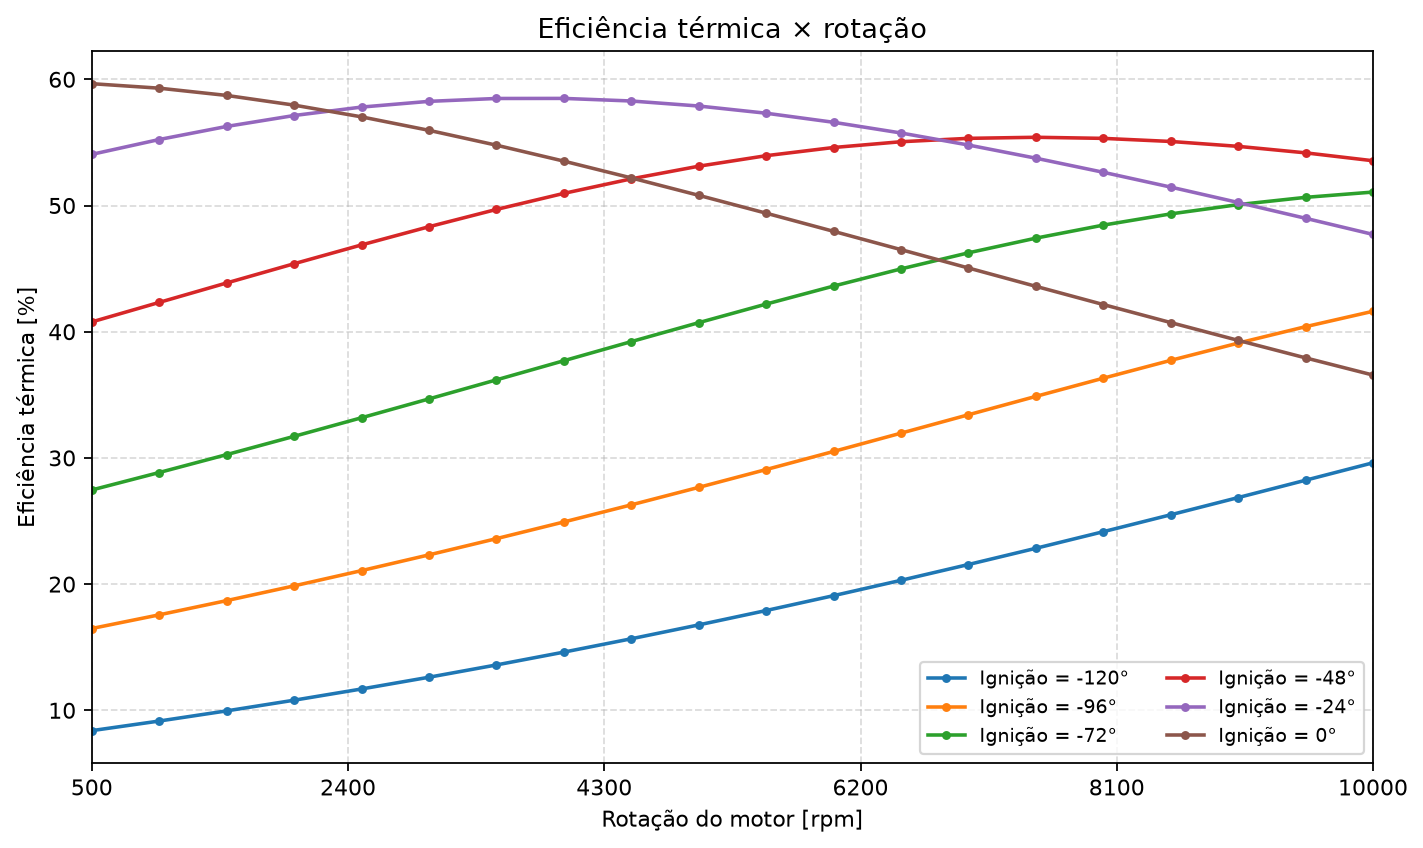
\includegraphics[width=\linewidth]{thermal_efficiency_vs_engine_speed.png}
\end{minipage}\hfill
\begin{minipage}[t]{0.49\linewidth}
\centering
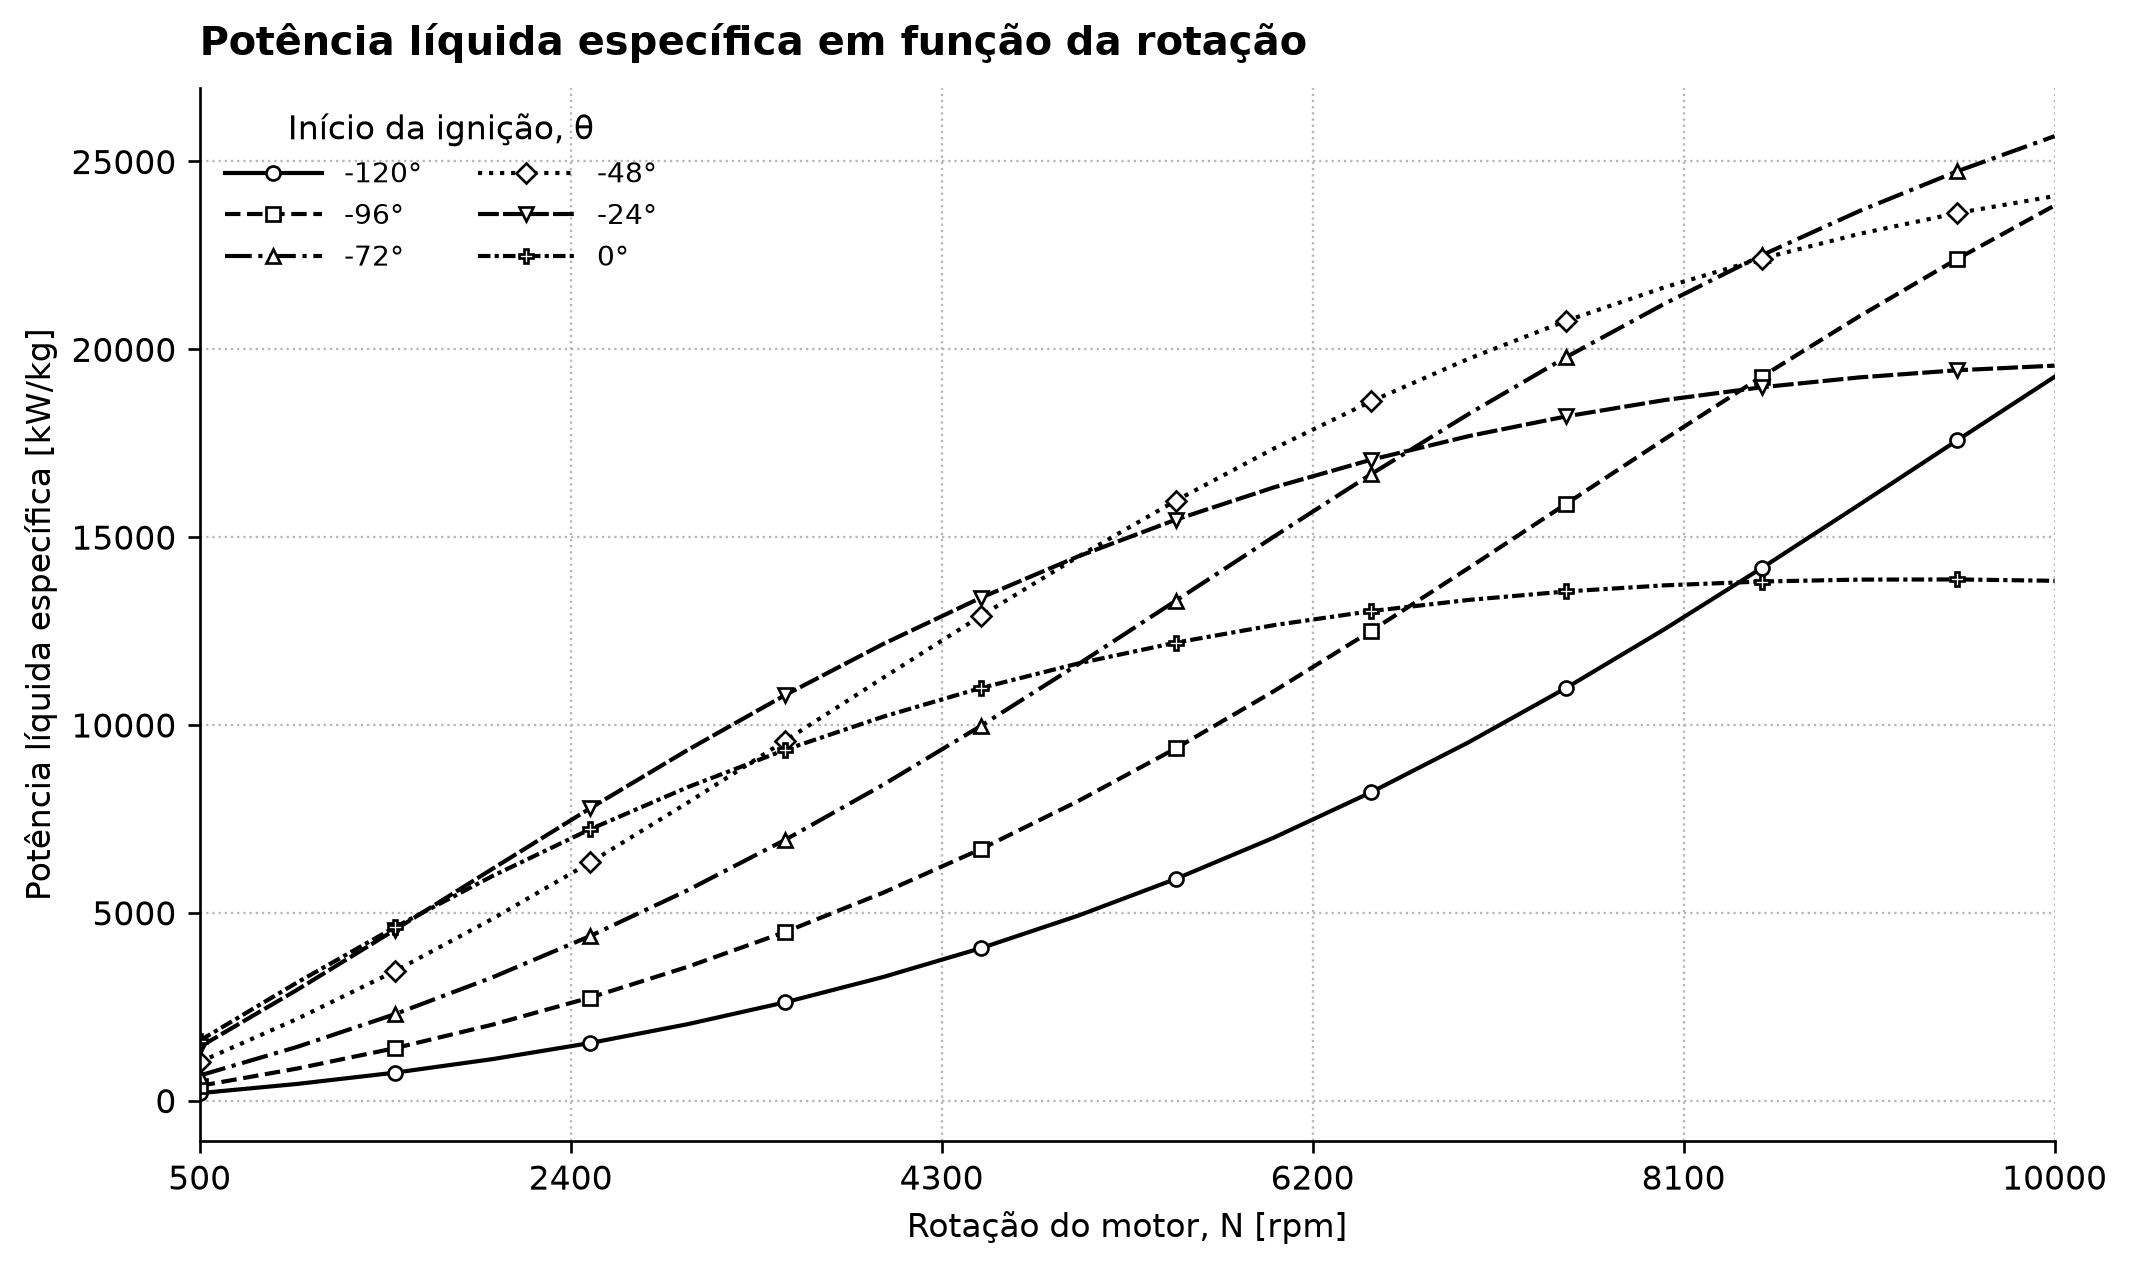
\includegraphics[width=\linewidth]{net_specific_power_vs_engine_speed.png}
\end{minipage}
\caption{Eficiência térmica e potência líquida específica na varredura de
rotação e instante de ignição. Traços e marcadores preservam a leitura em
escala de cinza.}
\label{fig:varredura-objetivos}
\end{figure}

\subsection{Desempenho do NSGA-III frente aos benchmarks}

A configuração-base C17 do NSGA-III foi avaliada frente aos três benchmarks.
As 84 execuções concluíram as 407\,232 avaliações previstas. O NSGA-II
apresentou o maior HV médio, $0{,}845957\pm0{,}000148$, apenas 0,004\% acima do
MOPSO e 0,116\% acima do NSGA-III. O MOPSO produziu o maior HV isolado,
0,847139. O MOEA/D teve HV médio 0,682\% abaixo do NSGA-II e consumiu 5,85
vezes mais tempo. Assim, os três primeiros métodos apresentaram qualidade
próxima, enquanto o NSGA-II teve a menor dispersão. Como não se aplicou teste
inferencial entre algoritmos, o benchmark é descritivo e não estabelece
superioridade estatística.

\begin{table}[htbp]
\centering
\caption{Desempenho da configuração-base do NSGA-III e dos benchmarks em 21 execuções.}
\label{tab:comparacao-algoritmos}
\small
\begin{tabular}{@{}lrrrr@{}}
\toprule
\textbf{Método} & \textbf{HV médio $\pm$ DP} & \textbf{Melhor HV} &
\textbf{Frente média} & \textbf{Tempo [s]} \\
\midrule
NSGA-II  & $\mathbf{0{,}845957\pm0{,}000148}$ & 0,846259 & 46,24 & $\mathbf{23{,}87\pm2{,}39}$ \\
NSGA-III (C17) & $0{,}844977\pm0{,}000755$ & 0,846350 & 47,29 & $25{,}16\pm2{,}75$ \\
MOPSO    & $0{,}845922\pm0{,}000717$ & \textbf{0,847139} & 191,95 & $23{,}89\pm1{,}95$ \\
MOEA/D   & $0{,}840189\pm0{,}004676$ & 0,844662 & 47,57 & $139{,}55\pm3{,}19$ \\
\bottomrule
\end{tabular}
\end{table}

O tamanho da frente do MOPSO decorre também de seu arquivo externo de até 192
soluções e não é diretamente comparável à população final dos demais métodos.
A Figura~\ref{fig:pareto-algoritmos} exibe a execução de maior HV de cada
método; a tabela das 21 repetições, e não apenas essa figura, fundamenta a
comparação de robustez. Todas as aproximações recuperaram o conflito esperado:
a eficiência máxima da união foi 38,434\% em 500,0 rpm,
$\theta=-3{,}652^\circ$, $r=12{,}0000$ e $L/R=4{,}3730$, com
1\,601,5 kW/kg, ao passo que a potência máxima foi 25\,583,0 kW/kg em
10\,000,0 rpm, $\theta=-70{,}912^\circ$, $r=12{,}0000$ e
$L/R=4{,}4000$, com eficiência de 30,700\%.

\begin{figure}[htbp]
\centering
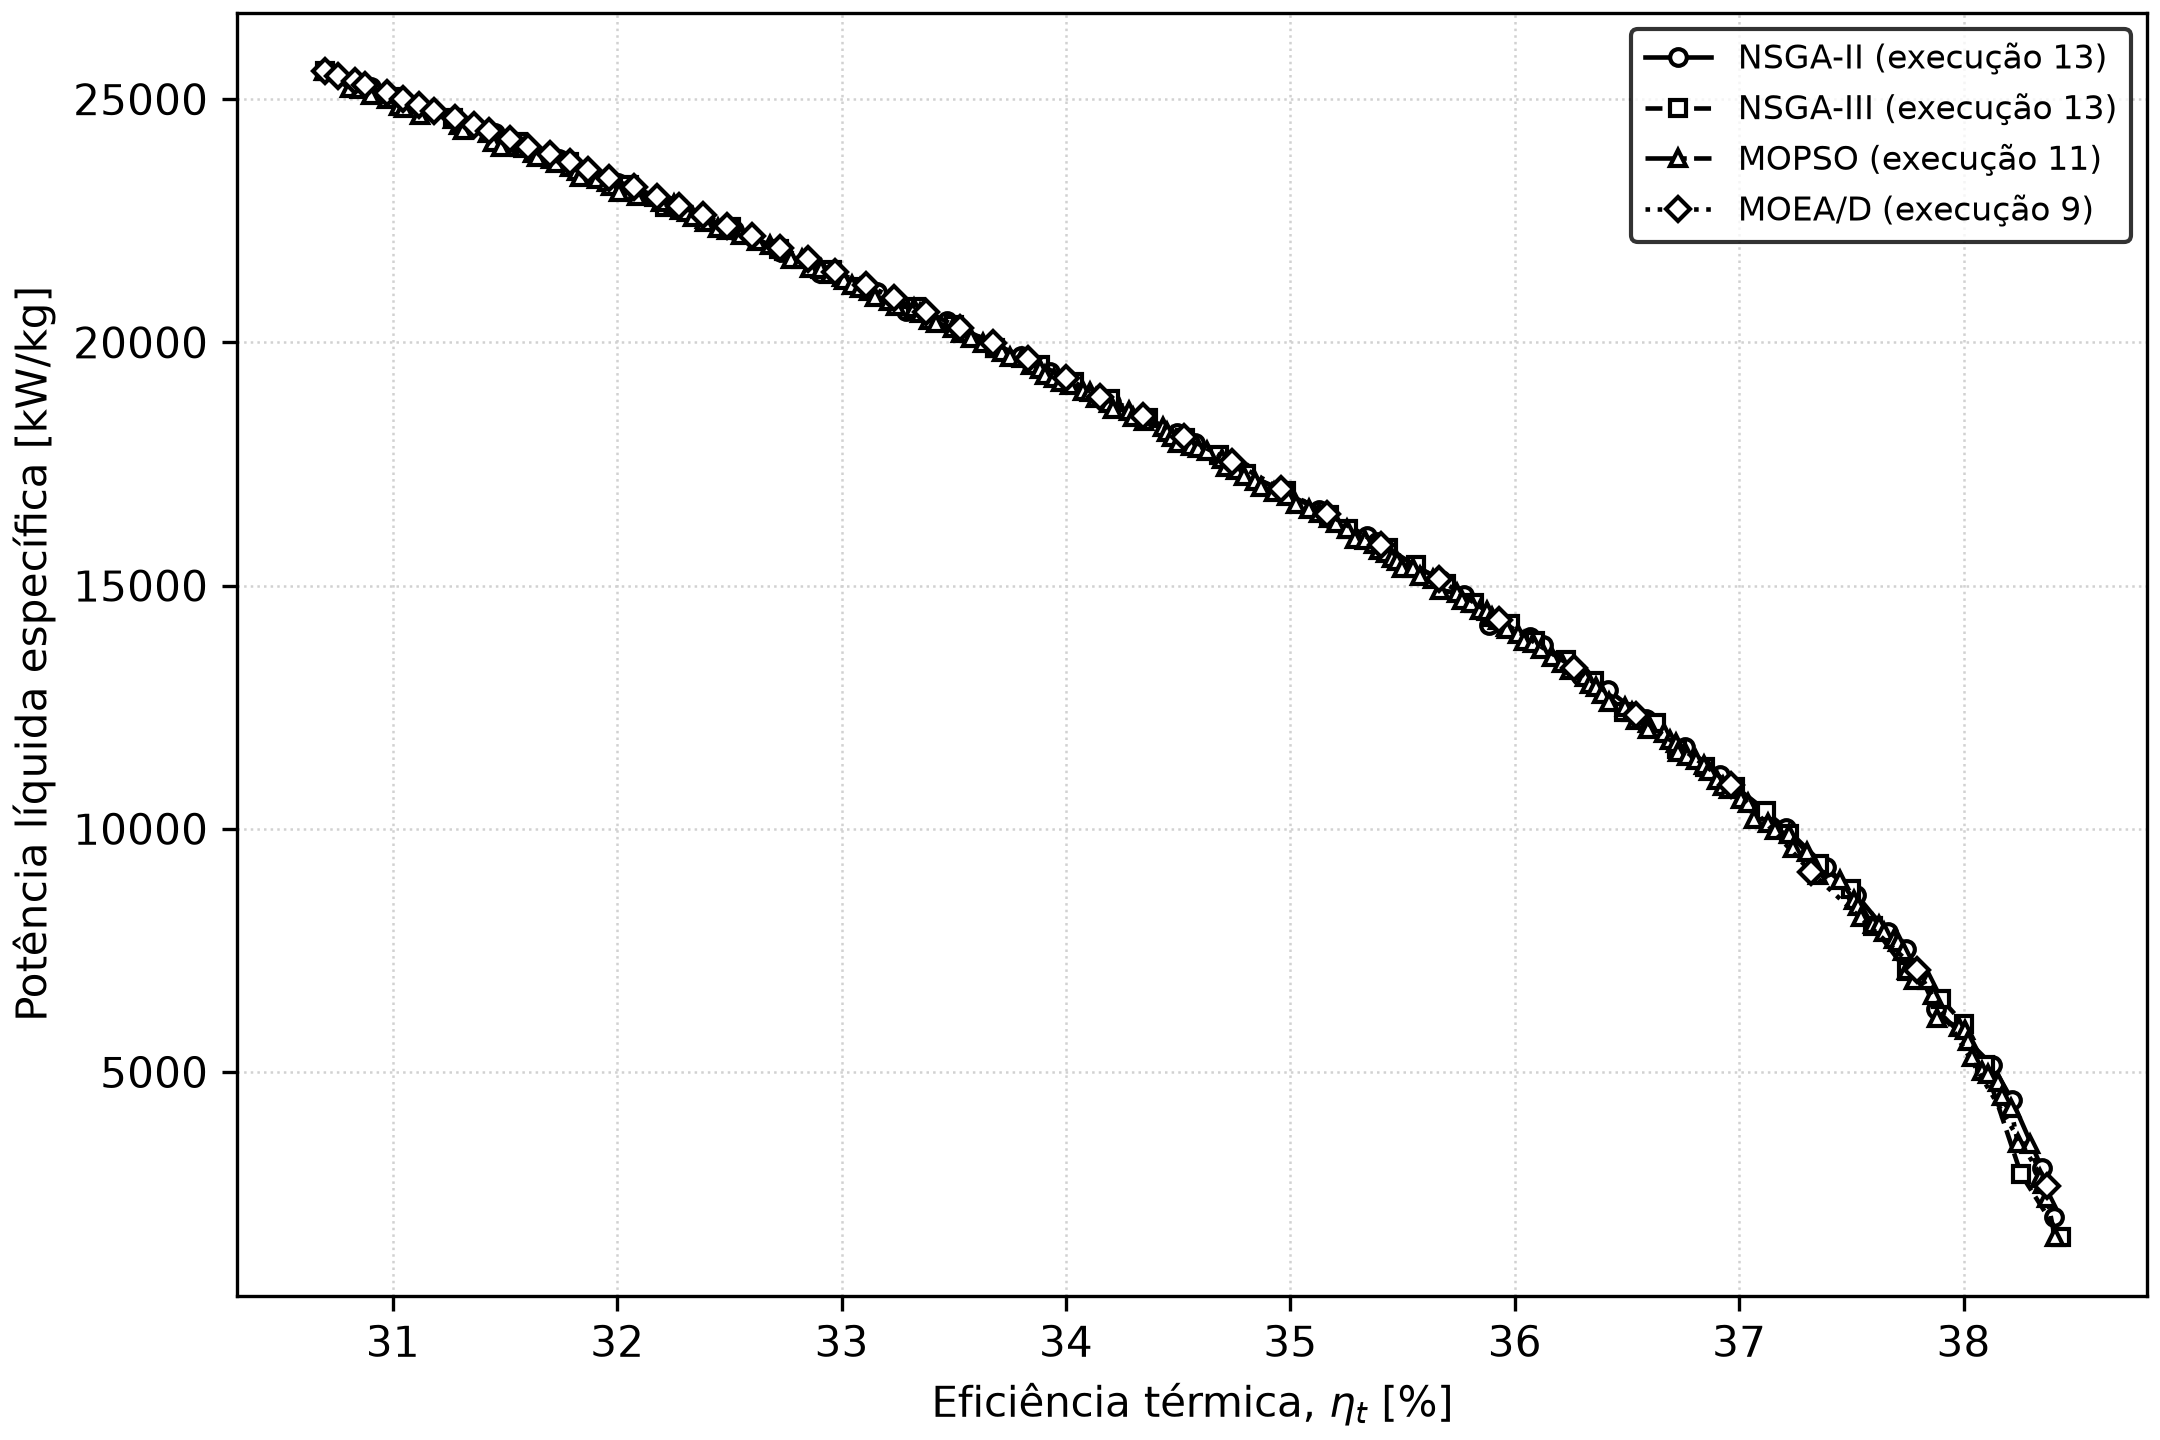
\includegraphics[width=0.88\linewidth]{multiobjective_pareto_front.png}
\caption{Frente do NSGA-III e frentes dos benchmarks nas execuções de maior
hipervolume. Traços e marcadores permitem impressão em preto e branco.}
\label{fig:pareto-algoritmos}
\end{figure}

\begin{figure}[htbp]
\centering
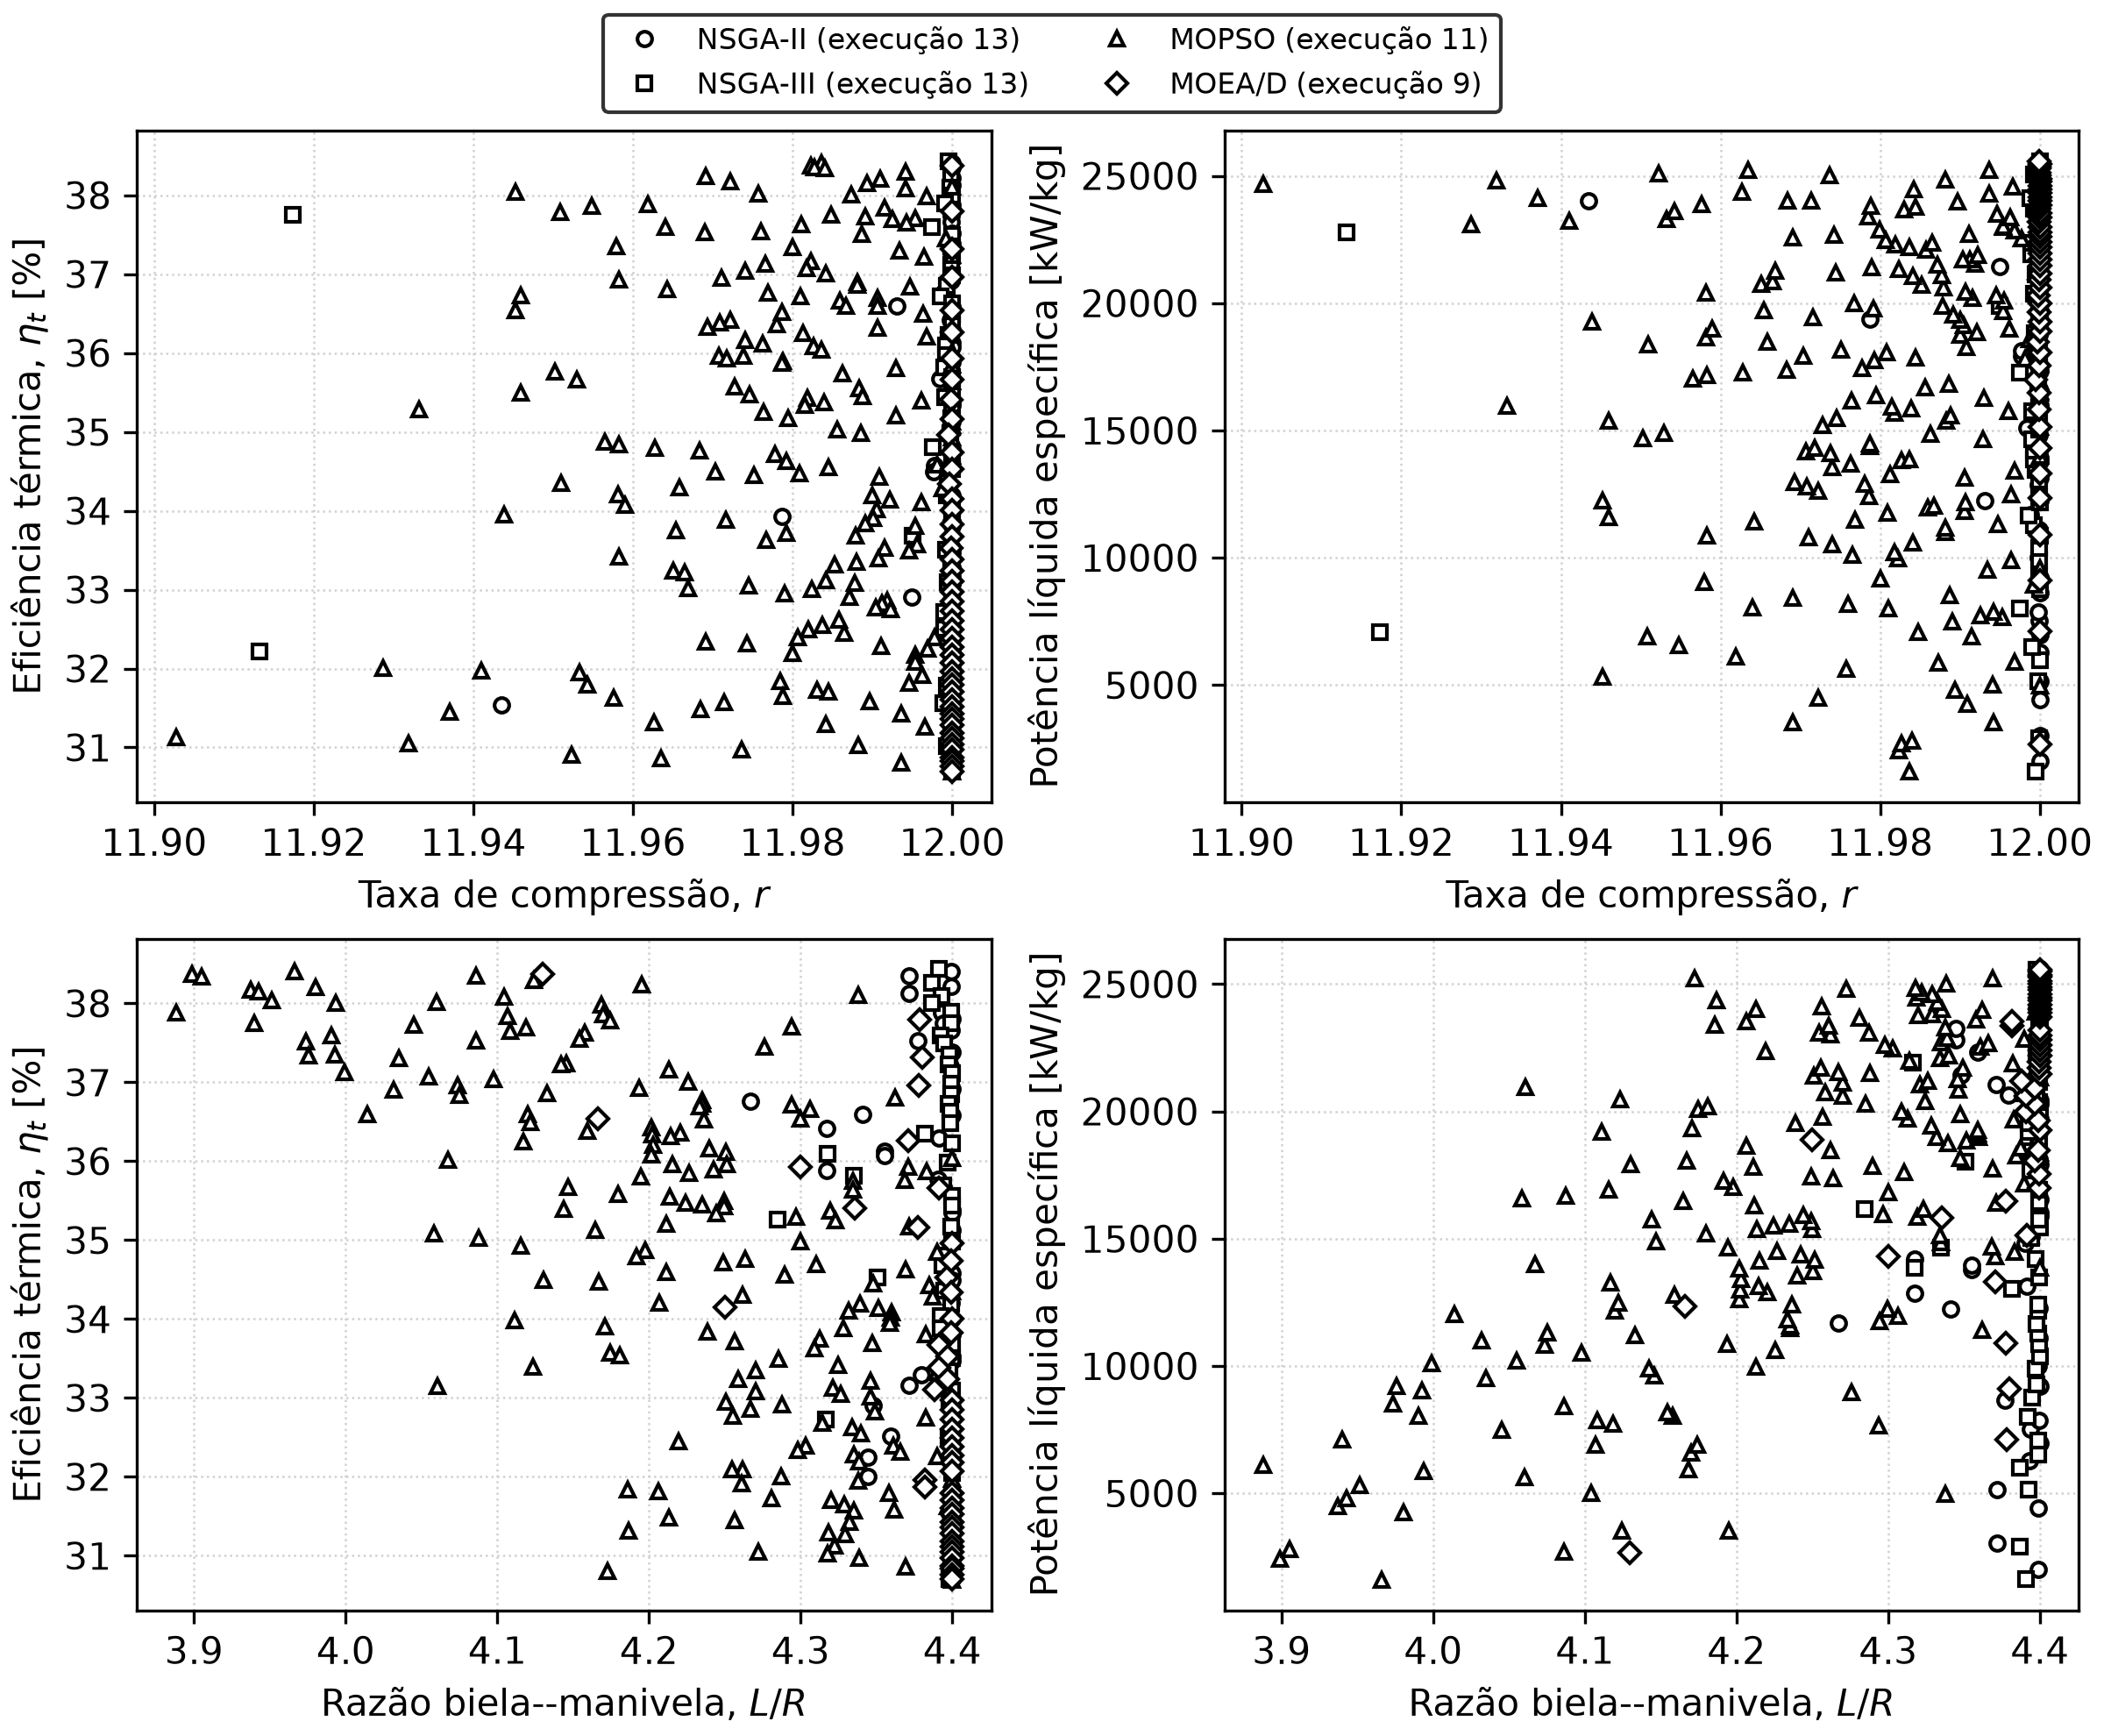
\includegraphics[width=0.94\linewidth]{multiobjective_constructive_decisions.png}
\caption{Taxa de compressão e razão biela--manivela nas frentes de maior
hipervolume de cada método, relacionadas aos dois objetivos.}
\label{fig:decisoes-construtivas}
\end{figure}

O melhor compromisso do NSGA-III apresentou escore 0,398451. Os benchmarks
localizaram soluções na mesma região física: 5\,226--5\,261 rpm, $\theta$
entre $-38{,}19^\circ$ e $-37{,}41^\circ$, $r$ entre 11,9992 e 11,9999,
$L/R$ entre 4,289 e 4,400, $\eta_t$ entre 35,507\% e 35,528\% e potência
entre 15\,471,3 e 15\,566,8 kW/kg. Seus escores foram 0,398507 (NSGA-II),
0,399447 (MOPSO) e 0,398533 (MOEA/D), diferenças pequenas e sem dominância
entre os compromissos do NSGA-III, NSGA-II e MOEA/D. O compromisso selecionado
do NSGA-III domina o do MOPSO, pois apresenta simultaneamente maior eficiência
e maior potência; essa comparação pontual não implica superioridade global de
sua frente ou do algoritmo. Nas médias das 21 repetições, os quatro métodos
também concentraram $r$ no limite superior. Essa tendência decorre do modelo
ar-padrão, que não representa detonação nem restrições mecânicas, e não deve ser
interpretada como recomendação direta de projeto.

\subsection{Situação do refinamento do NSGA-III}

O protocolo descrito na Seção~\ref{subsec:sensibilidade-nsga3} foi reformulado
para as quatro decisões e para o orçamento de 4\,848 avaliações por
configuração. Entretanto, a bateria correspondente ainda não foi executada.
Os arquivos \texttt{nsga3\_sensitivity\_*} atualmente versionados foram gerados
no estudo anterior, com duas decisões e 504 avaliações, e não são
metodologicamente comparáveis ao novo desenho. Por esse motivo, seus
identificadores de configuração, estatísticas e figuras são deliberadamente
omitidos deste artigo.

No novo desenho, C17 é apenas a configuração-base de 48 indivíduos e 100
gerações, não uma configuração recomendada. A recomendação dependerá das 252
execuções da triagem e das 70 execuções de confirmação, totalizando 322
execuções e 1\,561\,056 avaliações do FTHA. Somente após essa bateria será
possível identificar as três melhores configurações iniciais, confirmar seu
desempenho nas 14 sementes reservadas e estimar os efeitos dos hiperparâmetros.
Até então, não se atribui ganho de HV nem superioridade estatística a qualquer
configuração refinada.

\subsection{Limitações de interpretação}

Os limites e os ótimos devem ser interpretados dentro do modelo ar-padrão FTHA.
A formulação representa gás ideal, sistema fechado, processos internamente
reversíveis e adição finita de calor, mas não inclui detonação, cinética da
mistura, transferência de calor às paredes, atrito, bombeamento, vazamento,
enchimento, limites de pressão, tensões mecânicas ou emissões. A ausência de
detonação e restrições mecânicas pode conduzir $r$ ao limite superior; isso
caracteriza o modelo e não recomenda automaticamente essa taxa para um motor
real. De modo semelhante, o efeito de $L/R$ restringe-se à cinemática do
volume: massa da biela, forças laterais, atrito, altura do bloco e resistência
estrutural não são contabilizados. A otimização identifica, portanto,
tendências termodinâmicas e compromissos no domínio estudado, não um projeto
construtivo completo ou validado experimentalmente.

%%%%%%%%%%%%%%%%%%%%%%%%%%%%%%%%%%%%%%%%%%%%%%%%%%%%%%%%%%%%%%%
\section{Conclusões}\label{sec:conclusoes}

Este trabalho aplicou o NSGA-III à maximização da eficiência térmica e da
potência líquida específica do modelo Otto com adição finita de calor,
empregando NSGA-II, MOPSO e MOEA/D como benchmarks. A implementação reproduziu
as eficiências publicadas e a triagem de 3\,000 pontos confirmou o conflito
entre os objetivos no domínio de rotação, instante de ignição, taxa de
compressão e razão biela--manivela. Sob 4\,848 avaliações por execução, o
NSGA-III localizou a mesma região de compromisso dos comparadores e obteve HV
médio 0,116\% inferior ao NSGA-II; o MOPSO registrou o maior HV isolado. Sem
teste inferencial entre métodos, esses contrastes permanecem descritivos.

A inclusão de $r$ e $L/R$ transforma parâmetros antes fixos em decisões que
alteram diretamente o volume de folga e a cinemática do pistão. Os métodos
concentraram $r$ próximo do limite superior e favoreceram valores elevados de
$L/R$ nos compromissos. Como o modelo não representa detonação, transferência
de calor, atrito ou restrições estruturais, essas tendências caracterizam o
modelo ar-padrão e não constituem recomendações construtivas para um motor real.

Também foi definido um refinamento reprodutível do NSGA-III com orçamento fixo,
36 configurações balanceadas, sementes comuns na triagem e confirmação
independente. A bateria nova ainda não foi executada; consequentemente, os
resultados legados de C09 e C12 não sustentam conclusões no espaço de quatro
decisões e nenhuma configuração refinada é recomendada neste estágio. A
contribuição atual consiste no problema ampliado, no benchmark reprodutível e
no protocolo de refinamento, não em uma variante estrutural do NSGA-III.

As conclusões se restringem a um modelo idealizado, sem validação experimental,
com quatro decisões, dois objetivos e um único domínio e orçamento. As frentes
têm cardinalidades distintas, em especial devido ao arquivo externo do MOPSO,
e o benchmark não empregou sementes pareadas entre algoritmos. Como próximos
passos, deve-se executar a nova bateria de refinamento e comparar a configuração
selecionada diretamente aos benchmarks com sementes comuns e cardinalidades
compatibilizadas. Recomenda-se ainda incorporar perdas térmicas e mecânicas,
detonação e dados experimentais, além de tratar pressão, temperatura, torque e
emissões como objetivos ou restrições.

%%%%%%%%%%%%%%%%%%%%%%%%%%%%%%%%%%%%%%%%%%%%%%%%%%%%%%%%%%%%%%%

\bibliographystyle{sbpo}
\bibliography{exemplo-latex}


\end{document}
